\section{DNN-HMM}\label{sec:dnnhmm}
Let's now dive into the core elements of DNN-HMM approach for SI, describing the general idea and architecture, which will be described in detail in section \vref{sec:architecture}.

The basic idea behind DNN-HMM starts from the observation that Deep Neural Networks (DNNs) are more easily capable of learning advanced, non-linear statistical relationships from input data, require a lot less preprocessing compared to GMMs, and can even work with non-independent feature frames. That being said, it seems logical and worth trying to use a DNN as an emission function of an HMM, instead of a GMM.


\subsection{Deep Neural Network (DNN)}\label{subsec:dnn}
A Deep Neural Network (DNN) is an artificial neural network that employs more than one hidden layer between the input and output layers to classify an input pattern or, more generally, learn to approximate a target function $f$. In the presence of a classification problem, such as the SI problem, an attempt is made to discriminate a pattern $x$ based on a feature $y$, which can take value among $Q$ categories (also called classes), and the DNN estimates the class probabilities $p_j, j \in \{1, ..., Q\}$. The input features to a DNN do not require special attention to preprocessing, and in fact in audio processing one can range from raw frames of audio, to MFCCs/MFCCs \& deltas, to Mel's log-scaled spectrogram features. Figure \vref{fig:dnn0} shows an example neural network for classification tasks.

\begin{figure}
	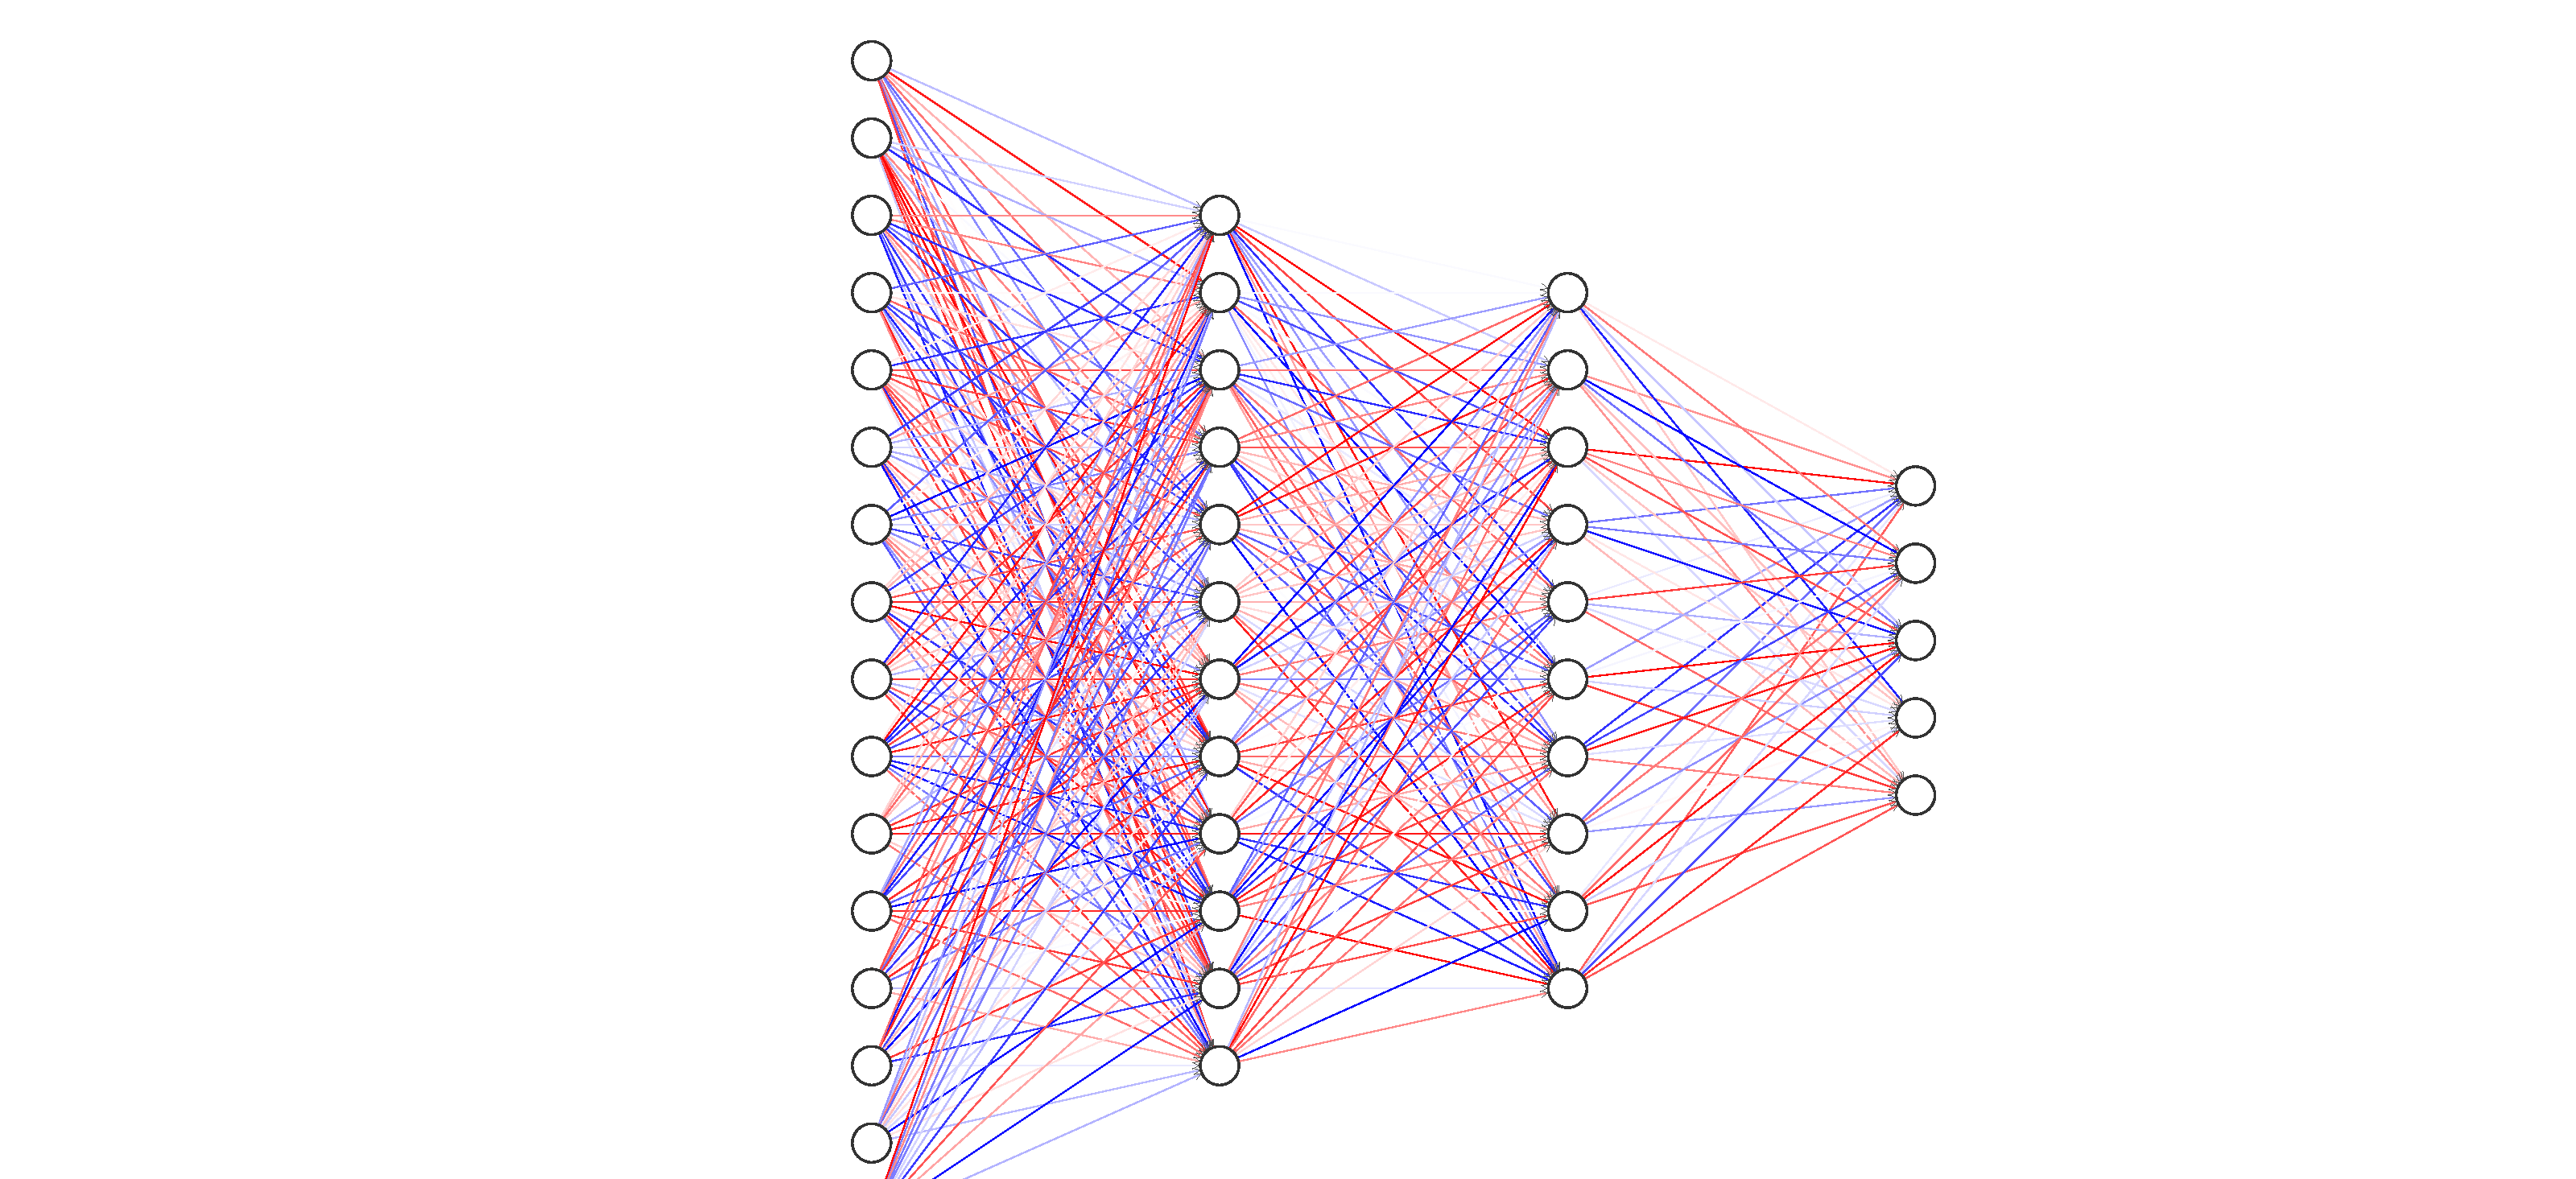
\includegraphics[width=0.5\textwidth]{images/nn}
	\caption{Deep neural network for classification with 5 output classes.}
	\label{fig:dnn0}
\end{figure}

More formally, a feed-forward DNN with $H$ layers, weight matrices $W_1, ..., W_H$, bias vectors $b_1, ..., b_H$ and activation functions $f_1, ..., f_H$ computes a non-linear function \cite{si:dnnhmm}:

$$g_{W, b}(x) := a_H(x) \text{ ,}$$
where, for $h = 1, 2, ..., H$: 

$$a_h(x) = f_h((a_{h-1}(x))^T \cdot W_h + b_h) \text{, and: }$$

$$a_0(x) = x$$
In classification tasks, the last layer activation function is often a softmax function $\sigma$, which outputs a probability $\hat{p}_j$ for each class $j$, and then the class with the highest probability is considered the predicted one:

$$q = \arg \max_j \hat{p}_j \text{, where: }$$

$$\hat{p}_j = f_H(x)_j = \sigma(x)_j := \frac{e^{x_j}}{\sum_{i=1}^{Q}e^{x_i}}$$

\paragraph{DNN training}
Generally speaking, DNN are trained to minimize a loss function $L(W, b)$ (e.g. mean squared error, mean absolute error or binary cross-entropy), and at each training cycle (so-called epochs), weights $W$ and biases $b$ are updated according to their gradient:

$$\nabla_{W, b}(L) = \Big[\frac{\partial L}{\partial b}, \frac{\partial L}{\partial W}\Big]^T \text{; }$$
while gradients are computed using the backpropagation algorithm \cite{backprogation}, the update rule for the weight based on their value can be done in many different ways, and it's in general considered a model hyperparameter to tune. Two notable and popular examples of optimization algorithms to update the network parameters are Stochastic Gradient Descent (SGD) \cite{sgd} and Adadelta \cite{adadelta}, which were also used to train the models for this work.

In multi-class classification tasks such as SI, the most used loss function is the categorical cross-entropy \cite{si:dnnhmm}:

$$L = \sum_{i=1}^{Q} p_j \log \hat{p}_j \text{, }$$
where $p_j$ is the target probability for class $j$ (usually 1 for right class, 0 otherwise) and $\hat{p}_j$ is the network-predicted probability for target class $j$.











\subsection{How DNN-HMM works}

\paragraph{DNN-HMM training}
In contrast to traditional DNN systems for IS, in those based on DNN-HMM, the network output classes do not correspond to the speakers to be identified, but to the states of each GMM-HMM acoustic model speaker generated \cite{si:dnnhmm}. As previously said, the state sequences computed from the speaker utterances with the Viterbi algorithm are used as labels for audio frames, therefore each neural network output corresponds to a GMM-HMM acoustic model state.
Hence, by minimizing the categorical cross-entropy loss function $C$ on the utterances of the training set and the corresponding labels, the network is trained to predict the posterior probabilities of each HMM state $k$, given the input audio feature frame $o_t$:

$$P(s_{t} = k \, | \, o_t)$$
In this way, the network can learn meaningful features that allow it to assign to an audio the states computed from the acoustic model of its speaker (and consequently discriminate from one speaker to another).

\paragraph{DNN-HMM decoding}
In testing stage, a new audio $o = o_1, ..., o_T$ from the test set is given as input to the neural network, which outputs a posterior probability $P(s_{t} = k \, | \, o_t)$ for each frame $o_t$. As briefly mentioned earlier, the idea behind DNN-HMM is that the neural network defines the emission probabilities of the HMM, so each posterior is converted into an emission probability (likelihood) using Bayes' theorem \cite{si:dnnhmm}:

$$e(o_t \, | \, s_{t} = k) = P(\, o_t | \, s_{t} = k) = \frac{P(s_{t} = k \, | \, o_t) P(o_t)}{P(s_{t} = k)}$$
In the previous formula, the prior probability $P(s_t = k)$ can be approximated by occurrences of state $k$ in the training utterances of the corresponding speaker, as relative frequency:

$$P(s_t = k) \approx \frac{\occurences(k)}{\statesspeakers \cdot \audiospeakers} $$
On the other hand, the (audio frame) prior probability $P(o_t)$ distribution is very hard to model without strong assumptions, but since all input frames are assumed to be independent each other, it can be considered as a constant scaling/normalization factor for the emission probability, and therefore ignored completely:

$$e(o_t \, | \, s_{t} = k) = P(\, o_t | \, s_{t} = k) = \frac{P(s_{t} = k \, | \, o_t)}{P(s_{t} = k)}$$
The last step in speaker identification task with DNN-HMM is the execution of the Viterbi decoding, where:

\begin{enumerate}[label=(\roman*), font=\itshape]
	\item $o = o_1, ..., o_T$ features against each speaker DNN-HMM model using the Viterbi algorithm, which uses the transition matrices $T_j$ and prior distributions $\pi_j$ of each speaker (from the GMM-HMM acoustic models), which gives in ouput a sequence of states $q_1, ..., q_T$ and its posterior probability:
	
	$$P_{\pi_j, T_j}(q_1, ..., q_T \, | \, o_1, ..., o_T) = \Viterbi_{P}^{\pi_j, T_j}(o)$$
	
	\item the audio is identified as belonging to the speaker DNN-HMM model which maximizes this probability:
	
	$$z^* = \arg \max_j P_{\pi_j, T_j}(q_1, ..., q_T \, | \, o_1, ..., o_T)$$
\end{enumerate}


